\section{MPI against the cached sequential program}
\label{sec:mpiresults}

\subsection{Method}

The MPI measurements were taken on \MpiMachine{} (Table~\ref{tab:environments}).
\MpiNodesSentence.

We tested $N = $~\MpiSizes{} with \MpiProcessCounts{} processes and a panel width of
$b = \MpiBlock$. The matrices are the assignment program's $A$ and $B$ for each size, built
from the same seed. \MpiRepeatsSentence, and we report medians. The MPI time runs from the
moment rank~0 starts handing out columns until rank~0 knows the determinant, so it includes
distributing the matrix. The sequential time is the assignment's elimination on the same
matrix, run by rank~0 in the same job while the other processes sleep. The two take turns
going first from one repetition to the next. Both work on the same matrix, so whichever
runs second finds the processor's caches warmed by the first, and for small matrices that
decides which one looks faster. In every measurement the MPI result and the sequential
result \MpiAllMatch.

\subsection{Break-even}

Table~\ref{tab:mpi} gives the times and Fig.~\ref{fig:mpispeedup} the ratio between them.
\MpiBreakEvenSentence. \MpiWinsSentence{} The best ratio we
measured is \MpiBestRatio{} at $N = \MpiBestRatioSize$.

\begin{table}[t]
  \caption{Median time for one determinant: the cached sequential program and the MPI
  program with $p$ processes. Each run times both on the same matrix, and the ratio is the
  median over the runs of sequential time divided by MPI time. Bold marks sizes at which MPI
  is faster.}
  \label{tab:mpi}
  \centering
  \footnotesize
  \setlength{\tabcolsep}{4pt}
  \begin{tabular}{@{}r r r r r r@{}}
\toprule
$N$ & Seq. & $p=1$ & ratio & $p=2$ & ratio \\
\midrule
10 & 1.25 $\mu$s & 1.83 $\mu$s & 0.64 & 6.00 $\mu$s & 0.32 \\
20 & 8.75 $\mu$s & 9.58 $\mu$s & 0.98 & 16.6 $\mu$s & 0.68 \\
30 & 32.5 $\mu$s & 30.6 $\mu$s & \textbf{1.04} & 41.9 $\mu$s & 0.89 \\
40 & 147 $\mu$s & 111 $\mu$s & \textbf{1.12} & 140 $\mu$s & \textbf{1.30} \\
50 & 303 $\mu$s & 250 $\mu$s & \textbf{1.17} & 261 $\mu$s & \textbf{1.26} \\
75 & 933 $\mu$s & 793 $\mu$s & \textbf{1.11} & 645 $\mu$s & \textbf{1.58} \\
100 & 1.89 ms & 1.72 ms & \textbf{1.08} & 1.02 ms & \textbf{1.78} \\
150 & 6.52 ms & 6.33 ms & \textbf{1.11} & 3.43 ms & \textbf{1.77} \\
200 & 14.1 ms & 13.1 ms & \textbf{1.15} & 7.53 ms & \textbf{1.80} \\
300 & 44.6 ms & 41.8 ms & \textbf{1.12} & 24.0 ms & \textbf{1.87} \\
400 & 100 ms & 94.3 ms & \textbf{1.09} & 53.1 ms & \textbf{1.97} \\
600 & 333 ms & 302 ms & \textbf{1.11} & 156 ms & \textbf{2.05} \\
800 & 759 ms & 738 ms & \textbf{1.07} & 418 ms & \textbf{2.02} \\
1000 & 1.47 s & 1.35 s & \textbf{1.09} & 735 ms & \textbf{2.15} \\
1500 & 4.88 s & 4.72 s & \textbf{1.02} & 2.42 s & \textbf{2.03} \\
2000 & 11.4 s & 11.3 s & \textbf{1.03} & 5.74 s & \textbf{1.99} \\
\bottomrule
\end{tabular}

\end{table}

\begin{figure}[t]
  \centering
  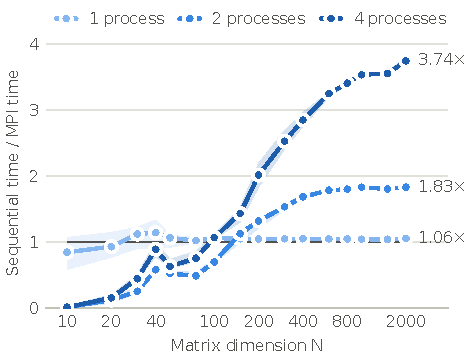
\includegraphics[width=\columnwidth]{figures/mpi_speedup.pdf}
  \caption{Sequential time divided by MPI time. Above the dark line at 1 MPI is faster.
  Each point is the median of the individual runs and the shaded band holds the middle half
  of them.}
  \label{fig:mpispeedup}
\end{figure}

For small matrices the fixed costs dominate. At the smallest sizes the arithmetic of a
determinant takes microseconds, less than it costs to hand the columns out and to send one
broadcast per panel. As $N$ grows, the arithmetic grows with $N^3$ while the number of
broadcasts grows with $N$ and their total size with $N^2$, so the messages matter less and
less.

The ratio could mix two effects, because the MPI program with a single process is not
the same code as the sequential program. It sends nothing, but it stores the matrix by
columns and eliminates one column at a time, where the assignment's elimination works row
by row. \MpiOneProcessSentence{} \MpiOneProcessWidthSentence{} The gain that comes from
the additional processes is the time with one process divided by the time with
\MpiMostProcesses, which is \MpiParallelGain{} at the largest size.

\subsection{Messages}

At $N = \MpiLargestSize$ with \MpiMostProcesses{} processes the run distributes
\MpiLargestDistributedMegabytes~MB of columns and then sends \MpiLargestPanels{} broadcasts
of \MpiLargestBroadcastMegabytes~MB in total.

\MpiBlockSentence{} That is the shape to expect. A panel that is wide compared with the
matrix leaves one process preparing most of the columns while the others wait, and a width
of one sends a broadcast for every column.

\begin{table}[t]
  \caption{Sequential time divided by MPI time for different panel widths $b$, with
  \MpiBlockProcesses{} processes. Higher is better. Bold marks the best width for each size.}
  \label{tab:blocks}
  \centering
  \footnotesize
  \begin{tabular}{@{}r r r r r r@{}}
\toprule
$N$ & $b=1$ & $b=4$ & $b=8$ & $b=32$ & $b=128$ \\
\midrule
100 & 0.30 & 0.83 & \textbf{1.07} & 0.81 & 1.01 \\
200 & 0.77 & 1.53 & \textbf{2.02} & 1.69 & 0.83 \\
400 & 1.75 & 2.68 & \textbf{2.85} & 2.54 & 1.29 \\
800 & 2.88 & 3.35 & \textbf{3.41} & 3.13 & 2.05 \\
1000 & 3.04 & 3.42 & \textbf{3.54} & 3.23 & 2.28 \\
\bottomrule
\end{tabular}

\end{table}
